\documentclass[preprint, 12pt]{elsarticle}
%\documentclass[letterpaper, 10 pt, conference]{ieeeconf}  % Comment this line out
                                                          % if you need a4paper
%\documentclass[a4paper, 10pt, conference]{ieeeconf}      % Use this line for a4
                                                          % paper

%\IEEEoverridecommandlockouts                              % This command is only
                                                          % needed if you want to
                                                          % use the \thanks command
%\overrideIEEEmargins

\usepackage{graphicx}
\usepackage{amsmath,amssymb} % define this before the line numbering.
\usepackage{lineno}
\usepackage{color}

%===========================================================
\usepackage{multirow}
\usepackage[tight,normalsize,sf,SF]{subfigure}

\usepackage{array} \newcommand{\vectornorm}[1]{\left|\left|#1\right|\right|}
\newcommand{\foreign}[1]{\emph{#1}}

\hyphenation{Bio-logic-ally-ins-pi-red}
%===========================================================

%\author{Anonymous Submission}
\journal{Image and Vision Computing Journal}

\begin{document}

\begin{frontmatter}

\title{
High-Throughput-derived Biologically-Inspired Features for Unconstrained Face Recognition
}

\author[rowland,mit]{Nicolas Pinto}
\ead{pinto@rowland.harvard.edu}

\author[rowland]{David D. Cox}
\ead{cox@rowland.harvard.edu}

\address[rowland]{The Rowland Institute at Harvard, Harvard University, Cambridge, MA 02142}
\address[mit]{McGovern Institute for Brain Research at MIT, Cambridge, MA 02139}


%===========================================================
\begin{abstract}
Many modern computer vision algorithms are built atop of a set of low-level
feature operators (such as SIFT \cite{sift,luo2007person}; HOG \cite{dalal2005hog,albiol2008face}; or LBP
\cite{ahonen2004face,ahonen2006face}) that transform raw pixel values into a representation better
suited to subsequent processing and classification.  While the choice of feature
representation is often not central to the logic of a given algorithm, the
quality of the feature representation can have critically important implications
for performance.  Here, we demonstrate a large-scale feature search approach to
generating new, more powerful feature representations in which a multitude of
complex, nonlinear, multilayer neuromorphic feature representations are randomly
generated and screened to find those best suited for the task at hand.  In
particular, we show that a brute-force search can generate representations that,
in combination with standard machine learning blending techniques, achieve
state-of-the-art performance on the \emph{Labeled Faces in the Wild (LFW)} \cite{huang:lfw}
unconstrained face recognition challenge set.  These representations outperform
previous state-of-the-art approaches, in spite of requiring less training data
and using a conceptually simpler machine learning backend.  We argue that such
large-scale-search-derived feature sets can play a synergistic role with other
computer vision approaches by providing a richer base of features with which to
work.

\end{abstract}

\begin{keyword}
face recognition \sep biologically-inspired
\end{keyword}

\end{frontmatter}


% Neuromorphic vision systems -- those that draw inspiration from the brain --
% have been demonstrated to be a powerful class of algorithms for a variety of
% face and object recognition tasks
% \cite{serre2007ror,mutch2008ocr,pinto:plos08,pinto:eccv08,jarrett-iccv-09}.

% We show that
% minor adjustment of the comparison function used can bring a simple,
% single-layer \emph{V1-like} model \cite{pinto:plos08} to within a few percent of
% state-of-the-art performance.  Further, by employing high-throughput screening
% and simple kernel blending techniques, we show that more sophisticated
% multi-layer architectures \cite{pinto:plos09} can achieve
% state-of-the-art performance.  To the extent that one accepts that the LFW set
% is a good surrogate for the problem of unconstrained face verification, these
% results show that our neuromorphic models are competitive with other
% state-of-the-art approaches, even without invoking particularly sophisticated
% machine learning techniques.  At the same time, we present an analysis of the
% errors made by our various models, and show that each of them makes appreciably
% the same errors, and that a large fraction of errors can be qualitatively
% explained by variation in the view of the targets. We argue that seriously
% tackling such image variation, and building sets that contain more real-world
% variation, will be an essential component of future research in unconstrained
% face recognition.


% -----------------------------------------------------------------------------
\section{Introduction}
% -----------------------------------------------------------------------------

Face recognition has long been, and continues to be, a highly active area of research \cite{belhumeur2002eigenfaces,yang2002kernel,vasilescu2002multilinear,zhao2003face,he2005face,hua2007face,hua2009robust,guillaumin2009you,hua2009robust,wright2009implicit,zou2007comparative}.
In recent years, interest in the problem of \emph{unconstrained} face
recognition has grown in the community, driven in large part by the creation of
the \emph{Labeled Faces in the Wild (LFW)} \cite{huang:lfw} test set, which has
provided a standardized benchmark against which to measure progress.  While
face recognition research \foreign{per se} has a long and rich history, much
work prior to the last decade was focused on face recognition in relatively
constrained environments (e.g. posed photographs, under controlled  lighting
conditions \cite{orl,yale,cvl,ar,phillips2000feret,gross2009multi}).  More
recently, thanks in large part to the rise of the internet, it has become
possible to assemble large collections of face images ``in the wild'' in the
sense that they come from a wide variety of sources and were not posed for the
purpose of research.  While this set has proven to be quite challenging, large
strides have been made in recent years towards higher performance
\cite{pinto:eccv08,pinto:cvpr09,taigman:bmvc09,wolf:accv09,kumar:iccv09,cao2010face}.

While a variety of different approaches to the \emph{LFW} set have been taken,
a common feature of most approaches is the use of some low-level visual feature
set, such as SIFT \cite{sift,luo2007person}; HOG
\cite{dalal2005hog,albiol2008face}; or LBP
\cite{ahonen2004face,ahonen2006face} that transforms raw pixels values into a
better form for subsequent processing.  While individual algorithms often do
not depend critically on the choice of a particular feature representation
used, the choice of features used does frequently play a key role in
determining performance.  Meanwhile, there are only a handful of visual feature
representations in common use, and arguably less attention has been paid to
developing new or better features.

One potentially promising source for new, more complex visual feature representations is the
class of ``biologically-inspired'' representations.
These approaches seek to build artificial visual 
systems that capture aspects of the computational architecture of the brain, in the hope of
eventually mimicking its computational abilities. Such efforts to model visual
computations done by the brain have a long history, at least dating back to
Fukushima's Neocognitron (1980; \cite{fukushima1980neocognitron}).  More recent
experiments with biologically-inspired models have shown them to be highly
competitive in a variety of different face and object recognition
contexts \cite{serre2007ror,mutch2008ocr,pinto:plos08,pinto:eccv08,jarrett-iccv-09}.

However, the range of possible feature representations that would count as ``biologically-inspired'' 
is broad, and it is not clear which particular instantiations of biologically-inspired
ideas are best for a given task.  Pinto et al. \cite{pinto:plos09} previously demonstrated a 
high-throughput screening approach for biologically-inspired algorithms, wherein a large
number of possible candidate models  from an inclusive model family are considered, 
and the best performing models are ``skimmed off the top'' 
and evaluated further.  However, while that work showed success with synthetic test 
images, it has not been known to date whether models from this class are competitive with 
current state-of-the-art approaches on standard face and object recognition test sets.

Here we present a modified large-scale feature search procedure that simplifies and accelerates the
search procedure described in \cite{pinto:plos09}, with the goal of generating feature
representations tailored for unconstrained face recognition, as embodied by the
\emph{LFW} test set.  Multiple complimentary representations are further derived through
training set augmentation, alternative face comparison functions, and feature set searches 
with a varying number of model layers.  These individual feature representations are then 
combined using kernel techniques to achieve even better performance.
We show that our approach yields multiple feature sets that 
outperform previous state-of-the-art approaches on the \emph{LFW} set,
even while requiring less training data and using simpler machine learning backends.
Finally, as a complement to experiments with natural face images, we characterize the tolerance of the resulting representations to various kinds of image transformations using rendered face images undergoing known view transformations.
In addition to providing evidence for the utility of large-scale feature search for standard 
``real world'' test sets, these results emphasize the value of good underlying 
representations and point a path forward in the generation of new, more powerful visual features.



%------------------------------------------------------------------------------
\section{Methods}
% -----------------------------------------------------------------------------


\begin{figure*}[ht]
\begin{center}
	\rule{1\linewidth}{0pt}
        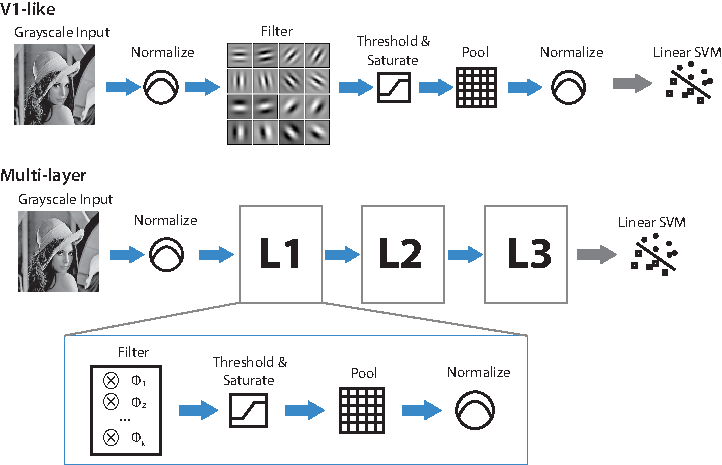
\includegraphics[width=1\linewidth]{figures/models_v2.pdf}
\end{center}
   \caption{{\bf A schematic diagram of the system architecture of the family of
       models considered.}  Each model consists of one to three feedforward
     filtering layers, with the filters in each layer being applied across the
     previous layer.}
\label{fig:models}
\end{figure*}



% -----------------------------------------------------------------------------
\subsection{Large-scale feature search framework}
% -----------------------------------------------------------------------------
\label{sec:feature_search}

The large-scale feature search approach used here consists of four basic components:
(1) a parametric family of feature representation, wherein key aspects of the behavior of the 
features are controlled by a fixed set of parameters, (2) a generation procedure for 
choosing models from the larger family to evaluate, (3) a screening procedure, run on 
each candidate feature representation, to determine which models to evaluate further
and (4) a validation procedure, using independent data, to evaluate the utility of representations found
during the screening procedure.

The approach we follow here is similar to that described in \cite{pinto:plos09},
with two important differences, which we describe briefly here, and detail in depth below.
First, Pinto et al. \cite{pinto:plos09} used an unsupervised learning procedure in 
order to learn certain model parameters from a pre-training video set.  Here, we dispense with 
this unsupervised learning procedure, instead opting for greatly speeded model generation, allowing
more model architectures to be evaluated per unit time.  Second, we used the \emph{LFW View 1} subset 
as a screening set.  Details of the model family considered, and generation, screening and validation  
procedures used are described below.


% -----------------------------------------------------------------------------
\subsection{Biologically-inspired visual representations}
% -----------------------------------------------------------------------------
\label{sec:models}

In our experiments, we used two basic classes of biologically-inspired visual 
representations, shown in Fig.
\ref{fig:models}. 

First, as a  control, we used \emph{V1-like}, a 
one-layer model characterized by a
cascade of linear and nonlinear processing steps and designed to encapsulate
some of the known properties of the first cortical processing stage in the
primate brain.  Our \emph{V1-like} implementation was taken without modification from
\cite{pinto:plos08,pinto:eccv08}.

Second, we used two and three layer models following the basic multi-layer model
scheme described in \cite{pinto:plos09}.  Briefly, these
models consist of multiple stacked layers of linear-nonlinear processing stages,
similar to those in the \emph{V1-like} model.  Importantly, in order to speed the
processing of these models, we disabled the unsupervised learning mechanisms described in
\cite{pinto:plos09} and instead used \emph{random} filter kernels drawn from a uniform
distribution.  Prior experience of our group and others \cite{jarrett-iccv-09}
has suggested that random filters can in many cases function surprisingly well
for models belonging to this general class. Details of each model class follow.


\subsection{``V1-like'' visual representation}

In the \emph{V1-like} representation, features were taken without additional
optimization from Pinto et al.'s \emph{V1S+} \cite{pinto:plos08}.  This visual
representation is based on a first-order description of primary visual cortex V1
and consists of a collection of locally-normalized, thresholded Gabor wavelet
functions spanning a range of orientations and spatial frequencies.

% \emph{V1-like} features have been proposed by neuroscientists as a ``null''
% model (a baseline against which performance can be compared) for object and face
% recognition since they do not contain a particularly sophisticated
% representation of shape or appearance, nor do they possess any explicit
% mechanism designed to tolerate image variation (e.g. changes in view, lighting,
% position, etc. \cite{dicarlo:tics07,pinto:plos08}). Here, this model serves as
% a lower bound on the level of performance that can be achieved by only relying
% on relatively low-level regularities that exist in the test set.  To be
% considered a promising face recognition system in unconstrained settings, a
% model should minimally exceed the performance of the \emph{V1-like} model.

In spite of their simplicity, these features have been shown to be among the
best-performing non-blended features set on standard natural face and object
recognition benchmarks \cite{pinto:plos08,pinto:eccv08,pinto:cvpr09} (i.e. \emph{Caltech-101}\cite{feifei2007lgv},
\emph{Caltech-256}\cite{caltech256}, \emph{ORL}\cite{orl},
\emph{Yale}\cite{yale}, \emph{CVL}\cite{cvl}, \emph{AR}\cite{ar}, \emph{LFW}\cite{huang:lfw}) and are a key component of the
best blended solutions for some of these same benchmarks
\cite{gehler:iccv09}. We used the authors' publicly available source code to
generate these features and followed the same basic read-out/classification
procedure as detailed in \cite{pinto:plos08}, with two minor modifications.
Specifically, no PCA dimensionality reduction was performed prior to
classification (the full vector was used), and a different SVM regularization
parameter was used ($C=10^5$ instead of $C=10$, see below).

For a detailed description of the \emph{V1-like} visual representation, we refer
the interested reader to the methods of the original publication
\cite{pinto:plos08} and its source code.


\subsection{High-throughput-derived multilayer visual representations: \emph{HT-L2} and \emph{HT-L3}}

% In this study, we considered the five best two- and three-layer models generated
% from a high-throughput feature search procedure (model selection) for a total of 10
% multilayer visual representations.  An important feature of the generation of
% these representations, according to the basic scheme set forth in \cite{pinto:plos09},
% is the use of a massively parallel, high-throughput search over the parameter
% space of all possible instances of a large class of biologically-inspired
% models. Details of this model class and the high-throughput screening (model
% selection) procedure are modified from \cite{pinto:plos09} and are described below.

% --------------------------------------
\subsubsection{Model architecture: }

Candidate models were composed of a hierarchy of two (\emph{HT-L2}) or three
layers (\emph{HT-L3}), with each layer including a cascade of linear and
nonlinear operations that produce successively elaborated nonlinear feature-map
representations of the original image. A diagram detailing the flow of
operations is shown in Fig. \ref{fig:models}, and, for the purposes of notation,
the cascade of operations is represented as follows:

\begin{align*}
Layer^{0}: &\\ &\mathbf{Input}
\buildrel{\mathbf{Grayscale}}\over{\longrightarrow} \mathbf{ }
\buildrel{\mathbf{Normalize}}\over{\longrightarrow} \mathbf{N^{0}} %\\ Layer^{1}:
% &\\ &\mathbf{N^{0}} \buildrel{\mathbf{Filter}}\over{\longrightarrow}
% \mathbf{F^{1}} \buildrel{\mathbf{Activate}}\over{\longrightarrow} \mathbf{A^{1}}
% \buildrel{\mathbf{Pool}}\over{\longrightarrow} \mathbf{P^{1}}
% \buildrel{\mathbf{Normalize}}\over{\longrightarrow} \mathbf{N^{1}}
\end{align*}

and generally, for all $\ell \ge 1$:
\begin{align*}
Layer^{\ell}: &\\ &\mathbf{N^{\ell - 1}}
\buildrel{\mathbf{Filter}}\over{\longrightarrow} \mathbf{F^{\ell}}
\buildrel{\mathbf{Activate}}\over{\longrightarrow} \mathbf{A^{\ell}}
\buildrel{\mathbf{Pool}}\over{\longrightarrow} \mathbf{P^{\ell}}
\buildrel{\mathbf{Normalize}}\over{\longrightarrow} \mathbf{N^{\ell}}
\end{align*}

Details of these steps along with the range of parameter values included in the
random search space are described next.

% --------------------------------------
\subsubsection{Input and Pre-processing}

The input of the \emph{HT-L2} and \emph{HT-L3} models were 100x100 and 200x200
pixel images, respectively. In the pre-processing stage, referred to as
$Layer^{0}$, this input was converted to grayscale and locally normalized:

\begin{equation}\label{eq:input}
\mathbf{N^{0}=Normalize(Grayscale(Input))}
\end{equation}
where the $\mathbf{Normalize}$ operation is described in detail below.  Because
this normalization is the final operation of each layer, in the following
sections, we refer to $N^{\ell-1}$ as the input of each $Layer^{\ell>0}$ and
$N^{\ell}$ as the output.


% --------------------------------------
\subsubsection{Linear Filtering}

%\paragraph{ }
%\emph{Description:}
The input $N^{\ell-1}$ of each subsequent layer (i.e.  $Layer^{\ell}, \ell \in
\{1,2,3\}$) was first linearly filtered using a bank of $k^{\ell}$ filters to
produce a stack of $k^{\ell}$ feature maps, denoted $F^{\ell}$.  In a
biologically-inspired context, this operation is analogous to the weighted
integration of synaptic inputs, where each filter in the filterbank represents a
different cell.

%\emph{Definitions:}
The filtering operation for $Layer^{\ell}$ is denoted:
\begin{equation}
    \mathbf{F^{\ell} = Filter(N^{\ell-1}, \Phi^{\ell})}
\end{equation}
and produces a stack, $F^{\ell}$, of $k^{\ell}$ feature maps, with each map,
$F_{i}^{\ell}$, given by:
\begin{equation}\label{eq:filter}	
%F^{\ell}_i = N^{\ell-1} \otimes \Phi^{\ell}_i \qquad \forall i \in \{
F^{\ell}_i = N^{\ell-1} \otimes \Phi^{\ell}_i \quad \forall i \in \{
1,2,\dotsc,k^{\ell} \}
\end{equation}
where $\otimes$ denotes a correlation of the output of the previous layer,
$N^{\ell-1}$ with the filter $\Phi^{\ell}_i$ (e.g. sliding along the first and
second dimensions of $N^{\ell-1}$).  Because each successive layer after
$Layer^{0}$ is based on a stack of feature maps, $N^{\ell-1}$ is itself a stack
of 2-dimensional feature maps.  Thus, the filters contained within $\Phi^{\ell}$
are, in turn, 3-dimensional, with the their third dimension matching the number
of filters (and therefore, the number of feature maps) from the previous layer
(i.e. $k^{\ell-1}$).

%\paragraph{ }
\emph{Parameters:}
\begin{itemize}
\item The filter shapes ${f_s}^{\ell} \times {f_s}^{\ell} \times {f_d}^{\ell}$
  were chosen randomly with ${f_s}^{\ell} \in \{3, 5, 7, 9\}$ and
  ${f_d}^{\ell}=k^{\ell-1}$.
\item Depending on the layer $\ell$ considered, the number of filters $k^{\ell}$
  was chosen randomly from the following sets:
\begin{itemize}
\item In $Layer^{1}$, $k^{1} \in \{16, 32, 64\}$
\item In $Layer^{2}$, $k^{2} \in \{16, 32, 64, 128\}$
\item In $Layer^{3}$, $k^{3} \in \{16, 32, 64, 128, 256\}$
\end{itemize}
\end{itemize}
All filter kernels were fixed to random values drawn from a uniform
distribution.


% --------------------------------------
\subsubsection{Activation Function}

%\paragraph{ }
%\emph{Description:}
Filter outputs were subjected to threshold and saturation activation function,
wherein output values were clipped to be within a parametrically defined range.
This operation is analogous to the spontaneous activity thresholds and firing
saturation levels observed in biological neurons.

%\paragraph{ }
%\emph{Definitions:}
We define the activation function:
\begin{equation}
\mathbf{A^{\ell} = Activate(F^{\ell})}
\end{equation}
that clips the outputs of the filtering step, such that:
\begin{equation}\label{eq:activ}
	\mathbf{Activate(x)} = \left\{
	\begin{array}{ll}
		{\gamma_{max}}^{\ell} & \mbox{if $x >
                  {\gamma_{max}}^{\ell}$}\\ {\gamma_{min}}^{\ell} & \mbox{if $x
                  < {\gamma_{min}}^{\ell}$}\\ x& \mbox{otherwise}
	\end{array}
	\right.
\end{equation} 
Where the two parameters ${\gamma_{min}}^{\ell}$ and ${\gamma_{max}}^{\ell}$
control the threshold and saturation, respectively.  Note that if both minimum
and maximum threshold values are $-\infty$ and $+\infty$, the activation is
linear (no output is clipped).

%\paragraph{ }
\emph{Parameters:}
\begin{itemize}
\item ${\gamma_{min}}^{\ell}$ was randomly chosen to be $-\infty$ or $0$
\item ${\gamma_{max}}^{\ell}$ was randomly chosen to be $1$ or $+\infty$
\end{itemize}

\begin{figure*}[ht]
\begin{center}
	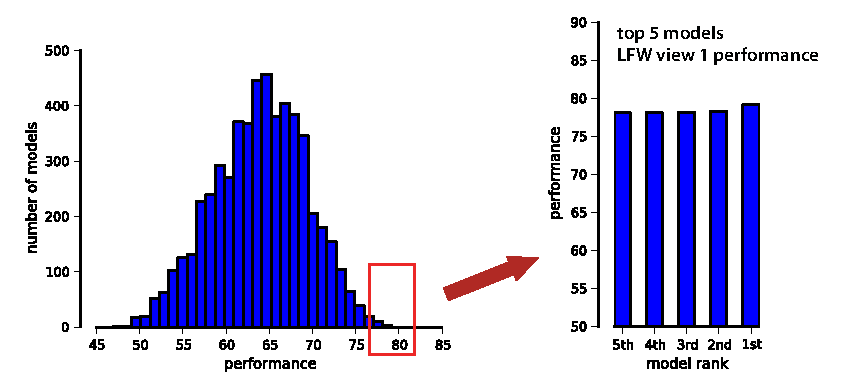
\includegraphics[scale=1]{figures/ht_process_l3.pdf}

    \caption[]{{\bf The high-throughput screening process used to find good representations.}  Here, data is shown for the screening of
      \emph{HT-L3} models.  A distribution of the performance of 6,917 randomly
      generated models is shown on the left, with the top five high-performing
      models replotted on the right.  Following screening, the models were evaluated
      exclusively with sets that do not overlap with the screening set.}

    \label{fig:ht_process}
 \end{center}
\end{figure*}


% --------------------------------------
\subsubsection{Pooling}

%\paragraph{ }
%\emph{Description:}
The activations of each filter within some neighboring region were then pooled
together and the resulting outputs were spatially downsampled.

%\paragraph{ }
%\emph{Definitions:}
We define the pooling function:
\begin{equation}
\mathbf{P^{\ell} = Pool(A^{\ell})}
\end{equation}
such that: \\
\begin{equation}\label{eq:pool}
\mathbf{P^{\ell}_{i}} = \mathbf{Downsample_{\alpha}}(
        \sqrt[p^{\ell}]{(A^{\ell}_i)^{p^{\ell}} \odot \mathbf{1}_{a^{\ell}
            \times a^{\ell}}} )
\end{equation}
, where $\odot$ is the 2-dimensional correlation function with
$\mathbf{1}_{a^{\ell} \times a^{\ell}}$ being an $a^{\ell} \times a^{\ell}$
matrix of ones ($a^{\ell}$ can be seen as the size of the pooling
``neighborhood'').  The variable $p^{\ell}$ controls the exponents in the
pooling function.

%\paragraph{ }
\emph{Parameters:}
\begin{itemize}
\item The stride parameter $\alpha$ was fixed to 2, resulting in a downsampling
  factor of 4.
\item The size of the neighborhood $a^{\ell}$ was randomly chosen from
  $\{3,5,7,9\}$.
\item The exponent $p^{\ell}$ was randomly chosen from $\{1, 2, 10\}$.
\end{itemize}
Note that for $p^{\ell}=1$, this is equivalent to blurring with a $a^{\ell}
\times a^{\ell}$ boxcar filter.  When $p^{\ell}=2$ or $p^{\ell}=10$ the output
is the $L^{p^{\ell}}$-norm
\footnote{The $L^{10}$-norm produces outputs similar to a \emph{max} operation
  (i.e. \emph{softmax}).}.



% --------------------------------------
\subsubsection{Normalization}

%\paragraph{ }
%\emph{Description:} 
As a final stage of processing within each layer, the output of the Pooling step
was normalized by the activity of their neighbors within some radius (across
space and across feature maps).  Specifically, each response was divided by the
magnitude of the vector of neighboring values if above a given threshold.  This
operation draws biological inspiration from the competitive interactions
observed in natural neuronal systems (e.g. contrast gain control mechanisms in
cortical area V1, and elsewhere \cite{geisler1992cni,rolls2002cnv})


%\paragraph{ }
%\emph{Definitions:}
We define the normalization function: 
\begin{equation}
\mathbf{N^{\ell} = Normalize(P^{\ell})}
\end{equation}
such that:
\begin{equation}\label{eq:norm}
N^{\ell} = \left\{ \scriptsize{
\begin{array}{ll}
  \rho^{\ell} \cdot C^{\ell} & \mbox{ if $ \rho^{\ell} \cdot
    \vectornorm{C^{\ell} \otimes \mathbf{1}_{b^{\ell} \times b^{\ell} \times
        k^{\ell}}}_2 < \tau^{\ell}$} \\ \frac{C^{\ell}}{\vectornorm{C^{\ell}
      \otimes \mathbf{1}_{b^{\ell} \times b^{\ell} \times k^{\ell}}}_2} &
  \mbox{otherwise}
\end{array}
} \right.
\end{equation}
with
\begin{equation}
C^{\ell} = P^{\ell}-\delta^{\ell} \cdot \frac{P^{\ell} \otimes
  \mathbf{1}_{b^{\ell} \times b^{\ell} \times k^{\ell}}}{b^{\ell} \cdot b^{\ell}
  \cdot k^{\ell}}
\end{equation}
Where $\delta^{\ell} \in \{0,1\}$, $\otimes$ is a 3-dimensional correlation over
the ``valid'' domain (i.e. sliding over the first two dimensions only), and
$\mathbf{1}_{b^{\ell} \times b^{\ell} \times k^{\ell}}$ is a $b^{\ell} \times
b^{\ell} \times k^{\ell}$ array full of ones.  $b^{\ell}$ can be seen as the
normalization ``neighborhood'' and $\delta^{\ell}$ controls if this neighborhood
is centered (i.e. subtracting the mean of the vector of neighboring values)
before divisive normalization.  $\rho^{\ell}$ is a ``magnitude gain'' parameter
and $\tau^{\ell}$ is a threshold parameter below which no divisive normalization
occurs.

%\paragraph{ }
\emph{Parameters:}
\begin{itemize}
\item The size $b^{\ell}$ of the neighborhood region was randomly chosen from
  $\{3,5,7,9\}$.
\item The $\delta^{\ell}$ parameter was chosen from $\{0,1\}$.
\item The vector of neighboring values could also be stretched by gain values
  $\rho^{\ell} \in \{10^{-1}, 10^{0}, 10^{1}\}$. Note that when $\rho^{\ell} =
  10^{0} = 1$, no gain is applied.
\item The threshold value $\tau^{\ell}$ was randomly chosen from $\{10^{-1},
  10^{0}, 10^{1}\}$.
\end{itemize}

% --------------------------------------
\subsection{Final model output dimensionality}
\label{sec:final_dim}

The output dimensionality of each candidate model was determined by the number
of filters in the final layer, and the x-y ``footprint'' of the layer (which, in
turn, depends on the subsampling at each previous layer).  In the model space
explored here, the possible output dimensionality ranged from 256 to 73,984.

% min = 256 = 1x1x256
% max = 73984 = 17x17x256 
% ( (((((((input-norm0-filt1-pool1)/2)-norm1-filt2-pool2)/2)-norm2-filt3-pool3)/2)-norm3) 
% = (((((((200-2-2-2)/2)-2-2-2)/2)-2-2-2)/2)-2) = 17)

% --------------------------------------
\subsection{Screening (model selection)}

A total of 5,915 \emph{HT-L2} and 6,917 \emph{HT-L3} models were screened on the \emph{LFW}
View 1 ``aligned'' set \cite{taigman:bmvc09}.  We selected the best five models
from each ``pool'' for further analysis on the \emph{LFW} View 2 set (Restricted
Protocol).  Note that \emph{LFW} View 1 and View 2 do not contain the same
individuals and are thus mutually exclusive sets. View 1 was designed as a model
selection set while View 2 is used as an independent validation set for the
purpose of comparing different methods.

Examples of the screening procedure for \emph{HT-L2} and \emph{HT-L3} models on the
\emph{LFW} View 1 task screening task are shown in Fig. \ref{fig:ht_process}.
Performance of randomly generated \emph{HT-L3} models ranged from chance performance
(50\%) to better than 80\% correct; the best five models were drawn from this
set and are denoted \emph{HT-L3-1st}, \emph{HT-L3-2nd}, and so on.  An analogous
procedure was undertaken to generate five two-layer models, denoted
\emph{HT-L2-1st}, \emph{HT-L2-2nd}, etc.



% --------------------------------------
\subsection{Evaluation Protocol}

To evaluate the performance of our biologically-inspired
representations, we followed the standard \emph{LFW} face verification
``Restricted View 2'' protocol.  6,000 different face image pairs (half
``same'', half ``different'') were drawn randomly from the sets and divided into
10-fold cross validation splits with 5,400 training and 600 testing examples
each.

Because the biologically-inspired representations used here generate one feature
vector per image, comparison functions were used to generate a new feature
vector for each pair, and these ``comparison'' features were used to train
binary (``same'' / ``different'') hard-margin linear SVM classifiers.  Following
\cite{pinto:cvpr09} we used the following element-wise comparison functions:
$|F_1 - F_2|$, $\sqrt{|F_1 - F_2|}$, $(F_1 - F_2)^2$, where $F_1$ and $F_2$
are the feature vectors generated from the first and the second image of the
pair, respectively.  We additionally added the comparison function $(F_1 \cdot
F_2)$, which was not used in \cite{pinto:cvpr09}, under the logic that it serves
as a soft ``AND''-like function (i.e.  it primarily results in a large response
for elements where both $F_1$ and $F_2$ are large). We hypothesized that such a
function would be valuable since our representations are all quite sparse, and
thus a coincidence of high feature values in common between the two test images
is likely to provide meaningful evidence of similarity.



\subsection{Kernel combinations and data-set augmentation}

While the high-throughput search techniques described above are capable of
yielding relatively high-performing individual representations for \emph{LFW} by
themselves, effectively all of the top-performing face recognition systems on
\emph{LFW} employ some form of more advanced machine learning backend to enhance
their performance \cite{taigman:bmvc09,wolf:accv09,kumar:iccv09,cao2010face}.  One common approach in this
regard is to blend together a large number of weak learners to produce
a blended classifier.

To explore what performance enhancement can be gained with modest amounts of
blending on top of our feature representations, we pursued a progressive strategy
of layering on additional kernels to produce successively larger and higher
performing blends. Two basic strategies were used for generating new kernels: 1)
feature augmentation, performing operations on the input image, such as cropping
and rescaling to produce alternate kernels using the same representation, and 2)
representation blending, that is, combining together kernels derived from
multiple separate feature representations (e.g. blending over the five
\emph{HT-L2} top models, or combining the top five \emph{HT-L2} and \emph{HT-L3}
models).

The progression of these additional elaborations is described below:

\subsubsection{Multiple rescaled crops}

Following \cite{pinto:cvpr09}, we augmented the dataset by computing features on
three different centered crops of the image: 250x250 (original), 150x150 and
125x75.  Each of these crops was resized to the standard input size of each representation,
and SVMs were trained separately for each crop size.
Blending of the resulting kernels was done by simple kernel addition, with each
kernel being trace-normalized (by the training kernel trace) prior to summation.
More sophisticated blending (e.g. IKL/MKL\cite{sonnenburg2006lsm},
LP-Boost\cite{gehler:iccv09}) were not used at this stage.

\subsubsection{Blending of the top 5 models within class}

While the top five models found by our high-throughput search all yield similar
levels of performance, they achieve this performance with different parameter
sets.  Consequently, to the extent that the top five models represent a
diversity of different ways to achieve good performance, we would expect that
blending these models would yield further enhancement of performance.  At this
stage, we combined all of the Stage 1 kernels above (multiple rescaled crops) from each of the top five
models within each model-class (e.g. \emph{HT-L2} and \emph{HT-L3}).

\subsubsection {Hierarchical blends across model class}

Finally, we also explored a more principled way to blend the representations
from each model class.  Following \cite{phow} we assigned exponentially larger
weight to higher-level representation (\emph{V1-like} $<$ \emph{HT-L2} $<$
\emph{HT-L3}) resulting in the following kernel: 

\begin{equation}
K(\cdot,\cdot) =
\displaystyle\sum_{\ell} (2^{\ell-1}) k_{\ell}(\cdot, \cdot)
\end{equation}

where $\ell=1$ for
\emph{V1-like} (one layer), $\ell=2$ for the top five \emph{HT-L2} (two layers)
and $\ell=3$ for the top five \emph{HT-L3} (three layers).

We note that the choice of blending strategies to consider on the View 2 set was 
driven by performance on the View 1 set, thereby avoiding selection bias artifacts.

\subsection{Additional Testing with Synthetic Face Images}

In order to assess model performance on an image set with a known amount of variation, 
we generated a set of 3D-rendered face images.  3D face meshes were randomly generated
using the FaceGen software package and were rendered using
the free POV-Ray ray-tracer.  For each rendered image, a model rotation 
(azimuth and elevation), position (x and y), and scale were drawn from a uniform 
distribution and the models were rendered with a common light source (Figure \ref{fig:variation_levels}).  
For the experiments presented here, rotation, size, and position were combined into
a single composite ``variation level'' wherein the variation in the pixel-level euclidean norm
was equalized for each kind of variation (e.g. one ``unit'' of rotation variation produced an
equivalent pixel-level change as one ``unit'' of position variation).  Examples of several
variation ``levels'' are shown in Figure \ref{fig:variation_levels}.

The rendered face/head was next composited onto one of four kinds of backgrounds: no
background, a white noise background, a phase-scrambled natural background 
(approximately equivalent to 1/f noise), and a randomly chosen natural background, chosen from
a large pool of outdoor background images (Figure \ref{fig:bg_variation}).  Care was taken 
to ensure that the same background image was never used in more than one final image.

\begin{figure*}[ht]
\centering 
\subfigure[\small{View, position an scale variation}]{
  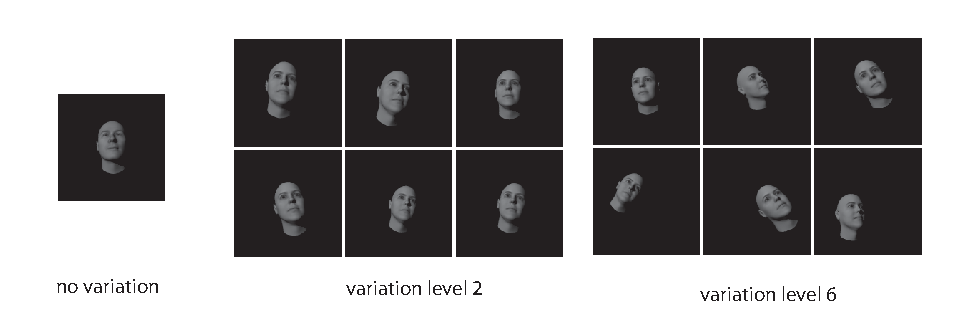
\includegraphics[scale=0.8]{figures/nongenerated/variation_level.pdf}
  \label{fig:variation_levels}
} 
\subfigure[\small{Background variation}]{
  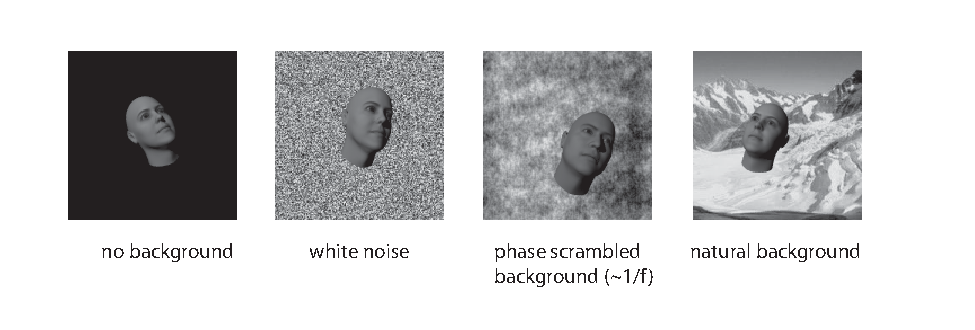
\includegraphics[scale=0.8]{figures/nongenerated/bg_variation.pdf}
  \label{fig:bg_variation}
} 
\caption[]{{\bf Synthetic face stimuli}}
\label{fig:synthetic_faces}
\end{figure*}


% -----------------------------------------------------------------------------
\section{Results}
% -----------------------------------------------------------------------------




\begin{table*}
\caption{Performance (\emph{LFW} Restricted View 2) of the family of biologically-inspired models and blends thereof.} 

\centering
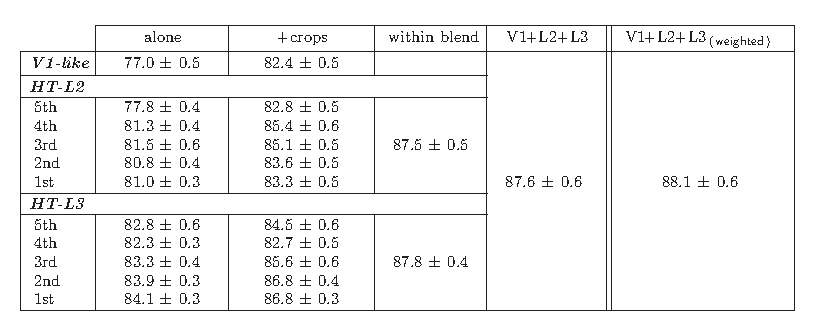
\includegraphics{tables/grand_performance_table_baked.pdf}

\label{tab:grand_performance_table}
\end{table*}





\subsection{High-throughput screening with \emph{LFW} View 1}

Fig. \ref{fig:ht_process} shows the results of high-throughput screening to select
model instantiations that are well-suited to the \emph{LFW} verification task.
For each model class, a multitude of models were randomly generated and
evaluated on the \emph{LFW} view 1 set, and the best five were selected for
further analysis.


\subsection{Performance on \emph{LFW} Restricted View 2}

Performance of individual models and model blends are shown in Table
\ref{tab:grand_performance_table}.  Performance ranging from 77.1 \% for the
simplest \emph{V1-like} model to 88.1\% for the largest blend were observed.  Taken
together, these results show that state-of-the-art level performance is possible
within the model family, and there exist multiple paths (e.g. based purely
on \emph{V1-like} models, and based on high-throughput, multi-layer models) to
achieving high levels of performance.  Fig. \ref{fig:roc_curves} shows
receiver-operator characteristic (ROC) curves for each of these models.

Interestingly, the inclusion of a single additional comparison function to the
\emph{V1-like} model blend described in \cite{pinto:cvpr09} brings an additional
3\% performance, placing it close to the last reported best performance on this
set, even without extensive blending.  Furthermore, we see that individual
\emph{HT-L3} models also perform surprisingly well --- coming to within a few percent correct of
the previous state-of-the-art.

A major advantage of our high-throughput approach is that it produces not one,
but a diversity of models, and this situation is ideally suited to kernel
blending approaches.  Once blending is added, especially when coupled with an
intelligent algorithm for weighting blended kernels, several different blends
achieved performance exceeding previously reported state-of-the-art values (see Table \ref{tab:table_soa}).  ROC
curves for various blend groupings are shown in Fig. \ref{fig:roc_curves}.

\begin{figure*}[ht]
\centering
\subfigure[\small{within-model-class blends}]{
  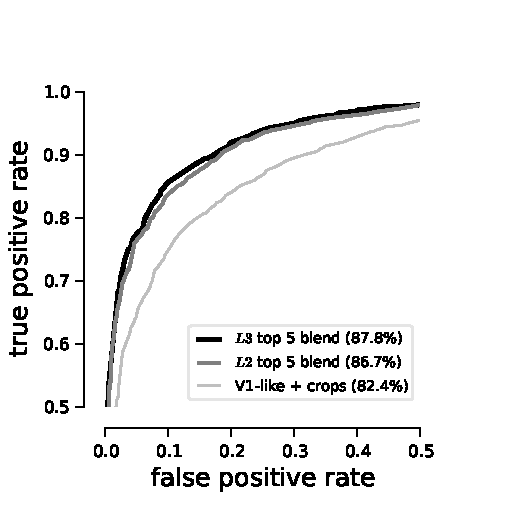
\includegraphics[scale=0.6]{figures/within_roc.pdf}
  \label{fig:within_rocs}
}
\subfigure[\small{across-model-class blends}]{
  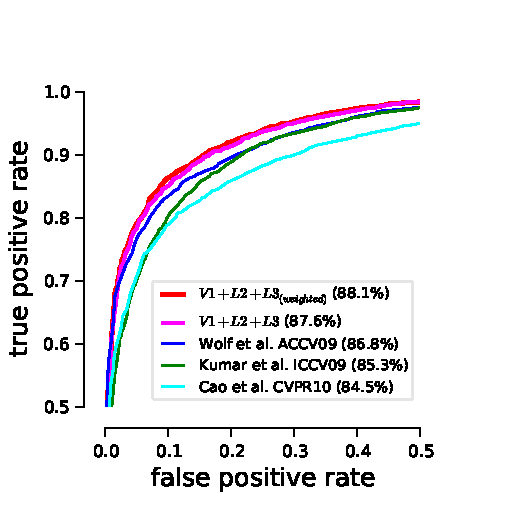
\includegraphics[scale=0.6]{figures/mega_blend_roc.pdf}
  \label{fig:megablend_rocs}
}

\caption[]{{\bf ROC curves for various model sub-families on \emph{LFW}
    Restricted View 2.} Curves for \cite{wolf:accv09}, \cite{kumar:iccv09} and \cite{cao2010face}
  are plotted in \ref{fig:megablend_rocs} for reference.  Plots are zoomed-in to
  facilitate comparison.}
\label{fig:roc_curves}
\end{figure*}


\begin{table}
\caption{Comparison with literature.} 

\begin{tabular}{|c||c|c|c|c|}
\hline
%Reference & Kumar et al. ICCV09 \cite{kumar:iccv09} & Wolf et al. ACCV09 \cite{wolf:accv09} & Cao et al. CVPR10 \cite{cao2010face} & This paper \\
 & Kumar et al. & Wolf et al. & Cao et al. & \\
Reference & ICCV09 & ACCV09 & CVPR10 & This paper\\
& \cite{kumar:iccv09} & \cite{wolf:accv09} & \cite{cao2010face} & \\
\hline\hline
Average error & 14.7\% & 13.2\% & 15.5\% & \bf{11.9\%} \\
& $\pm$1.2 & $\pm$0.3 & $\pm$0.5 & \bf{$\pm$0.6} \\
\hline
\end{tabular}
\label{tab:table_soa}
\end{table}



\begin{figure*}[ht]
  \centering \subfigure[Misses]{
    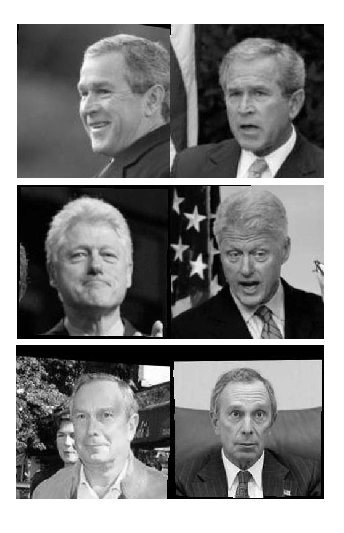
\includegraphics[scale=1]{figures/misses.pdf}
    \label{fig:misses}
  } \subfigure[False Positives]{
    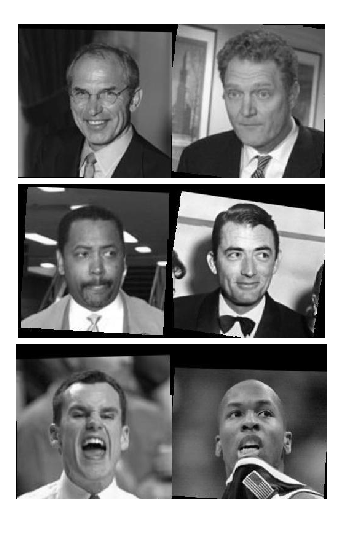
\includegraphics[scale=1]{figures/false_positives.pdf}
    \label{fig:false_positives}
  }
  \caption[]{{\bf Examples of common errors across models.} Misses tend to be
    dominated by differences in view, while false positives frequently occur when
    different individuals share a common view or expression. }
  \label{fig:error_examples}
\end{figure*}



\subsection{Analysis of Errors}

To understand better where room for improvement lies, we examined the error
trials (misses and false alarms) produced by each model for quantitative and
qualitative trends.  To determine whether different models were primarily making
the same or different errors, we segregated the responses of the \emph{V1-like}
and \emph{HT-L3} models (rescaled-crop augmented variants, see Methods) into
four categories: hits, misses, false positives, and correct rejections.  We then
computed the fraction of errors that these two models held in common and found
84.3\% of false positives were the same across the two models, and that
87.3\% of misses were missed by both models.  This high level of consistency
between error cases across the two models led us to ask whether a subset of
``hard'' images within the larger \emph{LFW} set could be driving errors and
capping performance.

Fig. \ref{fig:error_examples} shows examples of misses and false positives
held in common for both models.  While developing a quantitative framework
within which to analyze these errors is beyond the scope of this paper, several
patterns are evident, even upon casual inspection.  First, misses are dominated
by situations where the individual-to-be-matched is seen in non-frontal view in
at least one of the images.  Second, false positives appear to occur more often
in cases where different individuals appear in a very similar view, or with a
similar expression.


\subsection{Analysis of Tolerance to Variation, Using Synthetic Faces}

% -------------------------------------
%  Variation level figure
% -------------------------------------

\begin{figure}[ht]
    \centering
    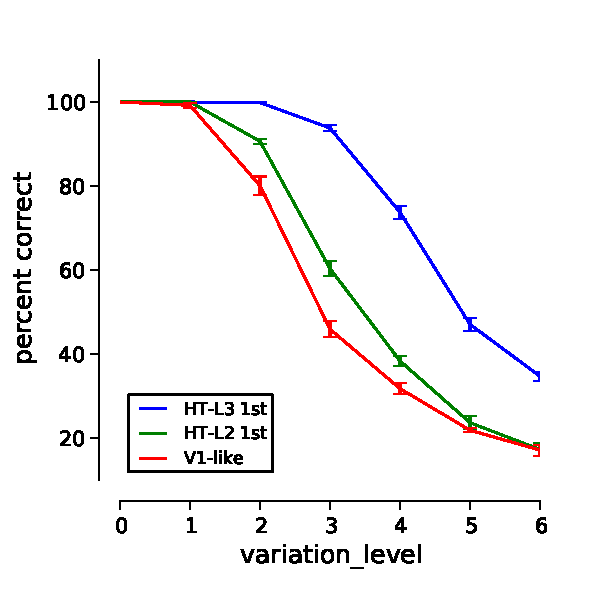
\includegraphics[scale=0.8]{figures/eight_faces_naturalbg_variation_v1like_a_plus.pdf}
    \caption[]{{\bf Model performance on synthetic faces as a function of level of variation.  Variation levels are described in detail in Section \ref{synthetic_methods}.}}
	\label{fig:perf_variation_levels}
\end{figure}

\subsubsection{Performance as a function of variation level}

The synthetic face evaluation sets used here provide us with the ability to parametrically control the level of rotation, position and scale variation that our models are required to tolerate.  Figure \ref{fig:perf_variation_levels} shows the performance the best models from each model class (V1-like, HT-L2, HT-L3) as a function of (composite) variation level for an eight-way face classification task.


\subsubsection{Effect of number of faces to be discriminated}

To further explore the behavior of our models with a controlled stimulus, we examined model
performance as a function of the number of faces to be discriminated.  In particular, we
considered cases with two, four, six, and eight faces.  Performance, grouped by model is shown
in Figure \ref{fig:nfaces_by_model}, and is shown grouped by variation level in
Figure \ref{fig:nfaces_by_variation}.  Predictably, absolute performance level is depressed as a larger
number of faces is considered, as is the chance performance level (dotted line). Interestingly, the
rate at which performance falls off varies between models as a function of both number of faces
to be discriminated, and as a function of variation level.  The stability of the performance of the
largest/deepest model --- HT-L3-1st --- is most pronounced when large number of faces and large amounts of variation
are considered.  Differences between models are far less pronounced with smaller numbers of
faces and lesser degrees of variation.

% -------------------------------------
%  N Faces Figure 2
% -------------------------------------

\begin{figure*}[ht!]
\centering
\subfigure[\small{V1-like}]{
  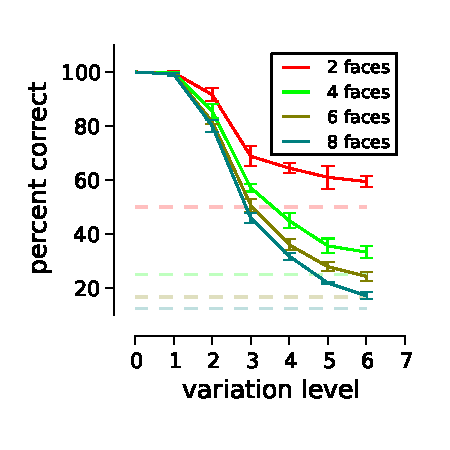
\includegraphics[scale=0.5]{figures/nfaces_variation_NaturalBg_v1like_a_plus.pdf}
  \label{fig:nfaces_v1like}
}
\subfigure[\small{HT-L2-1st}]{
  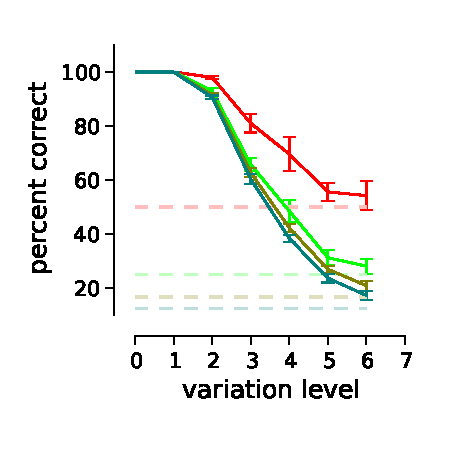
\includegraphics[scale=0.5]{figures/nfaces_variation_NaturalBg_ht1_1_l2_1st.pdf}
  \label{fig:nfaces_l2}
}
\subfigure[\small{HT-L3-1st}]{
  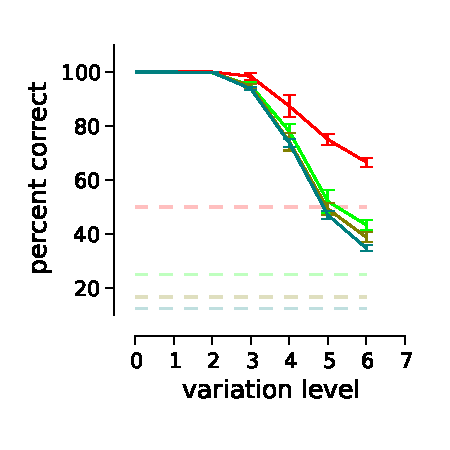
\includegraphics[scale=0.5]{figures/nfaces_variation_NaturalBg_ht1_1_l3_1st.pdf}
  \label{fig:nfaces_l3}
}
\caption[]{{\bf Effect of number of synthetic faces to be discriminated, sorted by model}}
\label{fig:nfaces_by_model}
\end{figure*}

% -------------------------------------
%  N Faces Figure
% -------------------------------------

\begin{figure*}[ht]
\centering
% \subfigure[\small{no variation}]{
%   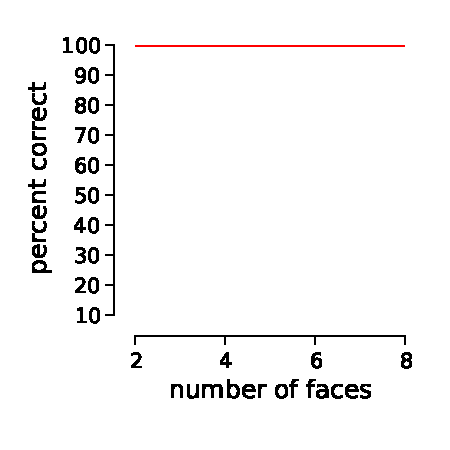
\includegraphics[scale=0.6]{figures/nfaces_variation0_by_model.pdf}
%   \label{fig:nfaces_var0}
% }
\subfigure[\small{variation level 2}]{
  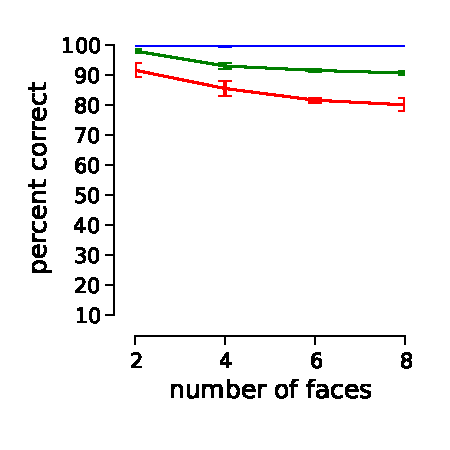
\includegraphics[scale=0.55]{figures/nfaces_variation2_by_model.pdf}
  \label{fig:nfaces_var2}
}
\subfigure[\small{variation level 4}]{
  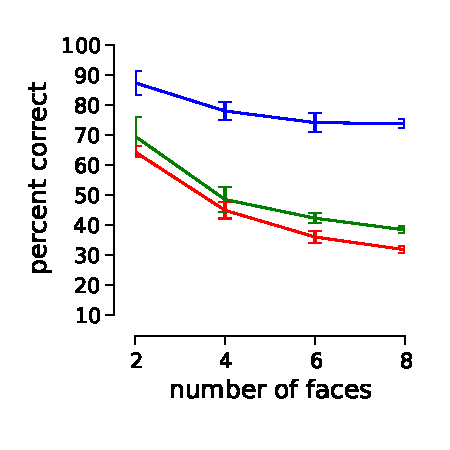
\includegraphics[scale=0.55]{figures/nfaces_variation4_by_model.pdf}
  \label{fig:nfaces_var4}
}
\subfigure[\small{variation level 6}]{
  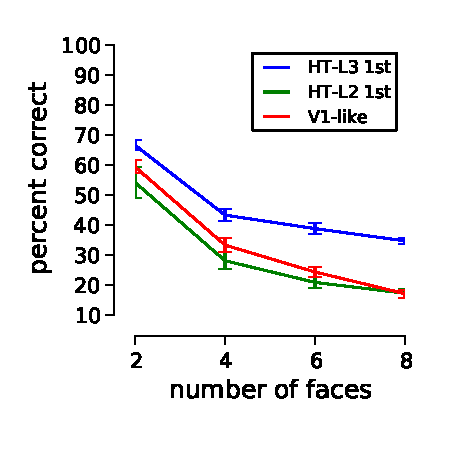
\includegraphics[scale=0.55]{figures/nfaces_variation6_by_model.pdf}
  \label{fig:nfaces_var6}
}

\caption[]{{\bf Effect of number of synthetic faces to be discriminated, sorted by variation level.} Note that the performance was 100\% in all cases for the zero variation condition (data not shown).}
\label{fig:nfaces_by_variation}
\end{figure*}


\subsubsection{Effect of background}

To explore the role of background variation, we evaluated model performance with four different background conditions: no background, white-noise background, phase-scrambled natural backgrounds (i.e. approx. 1/f noise), and natural backgrounds.  Performance as a function of background and variation level is shown in Figure \ref{fig:perf_bg_variation}.  Choice of background was found to have a profound effect on model performance.  In the absence of a background, the performance for most models remained high, even at relatively high levels of variation in view, position, and scale (e.g. greater than 90\% performance at variation level 4 for the HT-L3-1st and V1-like models).  However, the inclusion of any background resulted in a precipitous drop-off in performance for all models, except for the HT-L3-1st model, whose performance degraded gradually.  In general, progressively more realistic backgrounds proved increasingly difficult for all models.

% -------------------------------------
%  Effect of Background Figure
% -------------------------------------

\begin{figure*}[ht]
\centering
% \subfigure[\small{no variation}]{
%   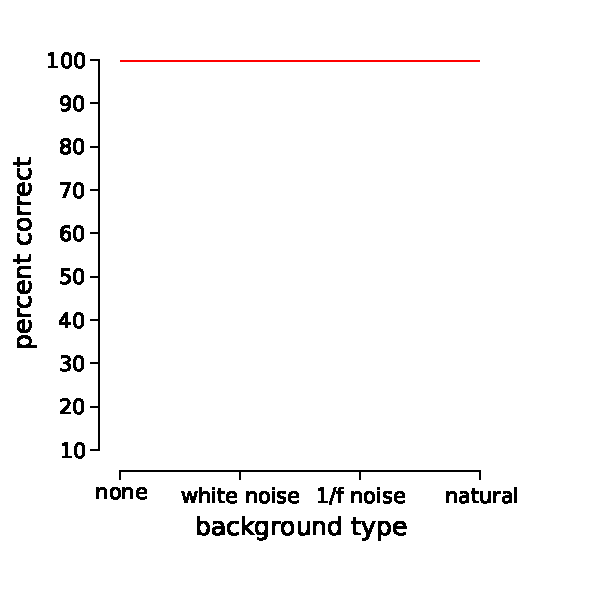
\includegraphics[scale=0.45]{figures/bg_variation0_by_model.pdf}
%   \label{fig:bg_var0}
% }
\subfigure[\small{variation level 2}]{
  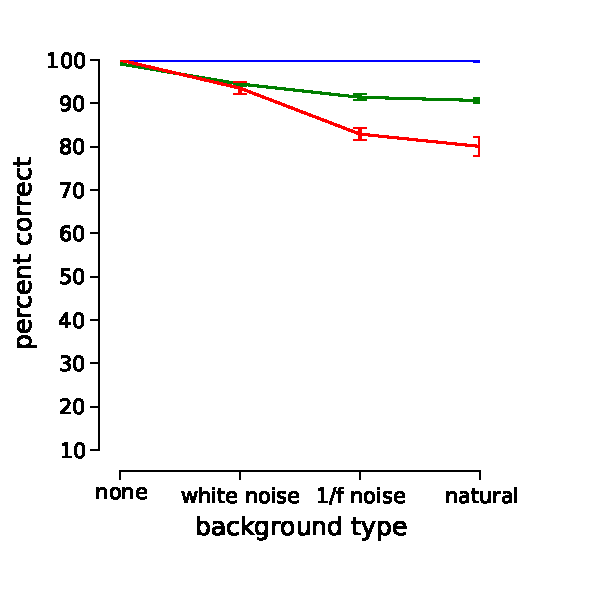
\includegraphics[scale=0.45]{figures/bg_variation2_by_model.pdf}
  \label{fig:bg_var2}
}
\subfigure[\small{variation level 4}]{
  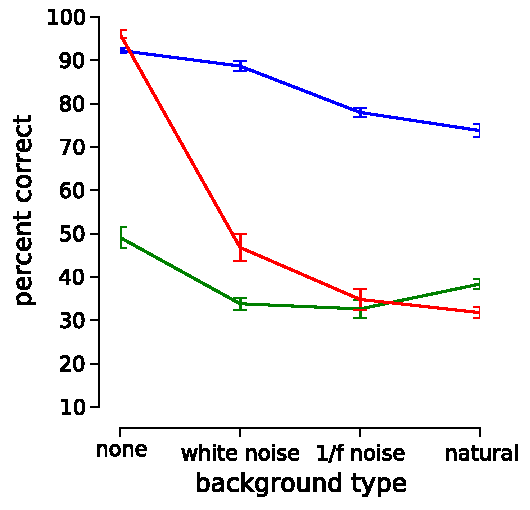
\includegraphics[scale=0.45]{figures/bg_variation4_by_model.pdf}
  \label{fig:bg_var4}
}
\subfigure[\small{variation level 6}]{
  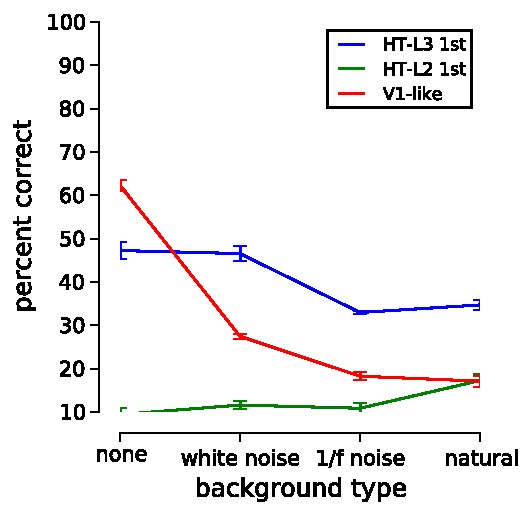
\includegraphics[scale=0.45]{figures/bg_variation6_by_model.pdf}
  \label{fig:bg_var6}
}

\caption[]{{\bf Effect of background type on performance with synthetic faces.} Note that the performance was 100\% in all cases for the zero variation condition (data not shown).  Example backgrounds from each class are shown in Figure \ref{fig:bg_variation}. }
\label{fig:perf_bg_variation}
\end{figure*}



% \subsection{Performance of models on a synthetic variation ``litmus test'' set}


% -----------------------------------------------------------------------------
\section{Discussion}
% -----------------------------------------------------------------------------


Our results provide more evidence that biologically-inspired models represent a promising
and powerful direction in face recognition research. Individual models from this
class are able to achieve good performance (e.g. around 77\% for \emph{V1-like} models,
84\% for \emph{HT-L3}), and blends of these models achieve more than 88\%
correct performance, placing it amongst the best performing systems on this challenge set.  
The model selection approach used here relies on a brute force search of a large space of candidate models, which is increasingly made feasible by the availability of recent advances in parallel computing resources, specifically graphics processing units (GPUs).  The roughly 15,000 models considered in this paper were evaluated in under one week.

Consistent with expectations, progressively more complex, multi-layer models are
able to outperform the simpler \emph{V1-like} model. Whether this higher
performance is due to a greater ability to tolerate image variation (one of the
original purposes for the construction of the \emph{HT-L3} model
class\cite{pinto:plos09}) or some other factor remains to be seen. It should be
noted that the \emph{HT-L2} and \emph{HT-L3} models used here were substantially
simplified from those present in \cite{pinto:plos09}, in that they did not have
structured filter kernels, nor were they subjected to any unsupervised learning.
Whether adding these features back will result in higher levels of performance
is an important future research question.  It should also be noted that, in terms of biological-inspiration, the model family tested here almost certainly represents just a small fraction of the complexity of the brain's visual system.  In addition, no claims are made that the three layers of the models presented here correspond in any strong way with the first three visual cortical areas.

While there still remains substantial room for improvement, concerns that
the \emph{LFW} set does not necessarily accurately reflect the ``full'' problem
of unconstrained face recognition
remain \cite{pinto:eccv08,pinto:cvpr09,kumar:iccv09}.  \emph{LFW} includes only
a handful of examples per individual, and these photographs were often taken in
the same setting and at the same event.  Furthermore, Kumar et
al. \cite{kumar:iccv09} showed that human observers were able to perform at
greater-than-90\% correct even when the faces themselves were masked out of the
test images, indicating that the backgrounds in the \emph{LFW} are more than
sufficient for solving the task at a level higher than the current machine state
of the art.

An analysis of the errors made by our models provides some clues about which
parts of the \emph{LFW} set are difficult and which ones are not.  Our models
failed on remarkably similar sets of face pairs, indicating that a common core
of ``hard'' images may exist within the larger \emph{LFW} set.  A striking,
albeit anecdotal, observation is that common error cases are dominated by misses
when the same individual is shown in differing views and by false positives
when two different individuals are compared while viewed from a similar angle
(e.g. Fig. \ref{fig:error_examples}).  An important feature of the \emph{LFW}
set is that faces must be detected by a Viola-Jones face detector in order to be
included in the set, and this effectively restricts the range of face views that
enter into the set (i.e. there is a bias towards frontal views).  We hypothesize
that those more off-axis views that do manage to pass the face detection filter
will present a particularly difficult challenge for a system trained on
the \emph{LFW} set.  The low-level (e.g. pixel-level) difference between two
different views of the same individual can easily be larger than the low-level
differences between two individuals in a similar pose.  A system that is not
specially designed to tolerate this kind of variation will have a high false
alarm rate on trials where two different individuals are seen in the same pose
and a high miss rate where the same individual is compared across different
poses.  At the same time, if the \emph{LFW} set contains a relatively small
fraction of these off-axis faces, then a system trained exclusively on
the \emph{LFW} set will face difficulty learning to tolerate these cases, even
if that system has the capability to learn such tolerance in principle.

At the same time, experiments with synthetic faces suggest that the underlying 
representations (particularly of the best three layer model) can indeed tolerate
significant variation in face pose, provided that adequately diverse training data
is available.  More generally, the steady progression towards larger 
and larger tolerance to variation when more processing layers are added to the 
model provides encouragement that hierarchical models such as these provide 
a promising path forward in the construction of transformation-invariant 
representations.

As continued research manages to chip away at the remaining ``performance gap''
between human and machines on the \emph{LFW} set, increased attention will need
to be paid to whether \emph{LFW} truly represents the problem of interest.  On
one hand, as long as some performance gap exists, the set is obviously valid at
a basic level.  However, the question remains whether a ``fuller'' formulation
of the problem (i.e. more natural, less filtered) might lead to faster progress.



% -----------------------------------------------------------------------------
\section{Acknowledgments}
% -----------------------------------------------------------------------------
The authors would like to thank Hanspeter Pfister, Wen-Mei Hwu, Vlad
Kindratenko and Jeremy Enos for making additional GPU clusters available for
this work. This work was funded by the Rowland Institute of Harvard, the NVIDIA
Graduate Fellowship, and the National Science Foundation (IIS 0963668).
Hardware support was generously provided by the NVIDIA Corporation.


\bibliographystyle{elsarticle-harv}
\bibliography{ivcj_lfw}

\end{document}
